\documentclass[tikz, border=1pt]{standalone}
\pdfoutput=1 % if your are submitting a pdflatex (i.e. if you have
             % images in pdf, png or jpg format)

\usepackage{graphicx}

% Use the tikz package
\usepackage{tikz}
\usetikzlibrary{decorations}


\begin{document}

        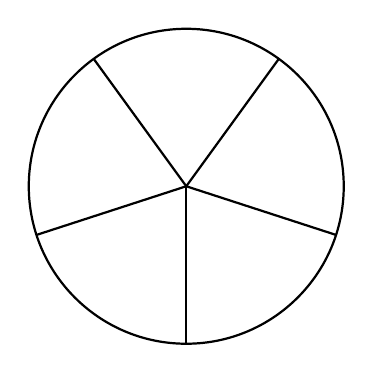
\begin{tikzpicture}
        
        
        \draw [thick] (0,0) circle (2);
        
        %axes
        %\draw[thick] (0,0) ++(72:2)--(0,0);
        \draw[thick] (0,0) ++(-90:2)--(0,0);
        %\draw[thick] (0,0) ++(144:2)--(0,0);
        \draw[thick] (0,0) ++(-162:2)--(0,0);
        %\draw[thick] (0,0) ++(216:2)--(0,0);
        \draw[thick] (0,0) ++(-234:2)--(0,0);
        %\draw[thick] (0,0) ++(288:2)--(0,0);
        \draw[thick] (0,0) ++(-306:2)--(0,0);
        %\draw[thick] (0,0) ++(0:2)--(0,0);
        \draw[thick] (0,0) ++(-18:2)--(0,0);
        
        \end{tikzpicture}

\end{document}
